% Copyright (c) 2021 Tobias Briones. All rights reserved.
% SPDX-License-Identifier: CC-BY-4.0
%
% This file is part of https://github.com/tobiasbriones/
% cp-unah-mm700-agricultural-soil-sampling-for-data-analysis
%
% This source code is licensed under the Creative Commons Attribution 4.0
% International License found in the LICENSE-CC file in the root directory of
% this source tree or at https://spdx.org/licenses/CC-BY-4.0

\subsection{Muestreo Estratificado}

Como se ha mencionado, este es uno de los temas centrales de esta investigación ya que los suelos agrícolas se pueden \textit{particionar} en lotes los cuales tienen atributos que permiten su medición y se espera poder llegar a establecerlos como homogéneos para poder elaborar el diseño del muestreo correspondiente.

\bigbreak

La población se debe de dividir (particionar) en \textbf{estratos} que sean disjuntos a dos. Esto viene de la clásica estratificación por capas. Así, para una población de tamaño $N$, se divide en $H$ estratos o capas con $N_h$ unidades en el estrato $H$. Es necesario conocer $N_1$, $N_2$, ... , $N_H$ y por tanto se tiene que $N_1 + N_2 + \cdot \cdot \cdot + N_H = N$.

\bigbreak

Para hacer un \textbf{muestreo estratificado aleatorio} como es de esperar, se toma cada estrato de $N_h$ unidades y se hacen $n_h$ mediciones aleatorias ($n_h < N_h$). Entonces el tamaño de todas las unidades de la población que se obtienen después de aplicar el muestreo se encuentra dado por $n = \sum \limits_{i=1}^H n_i$, este dato puede ser útil para dar la complejidad en espacio de la salida del muestreo virtual o de la entrada del modelo de analítica.

\bigbreak

Según la \textit{Guía de muestreo de suelo $\mid$ Gob.Pe} \cite{gobpe-ministerio-del-ambiente-2014}, el muestreo aleatorio estratificado se hace \say{cuando se dispone de información previa y el sitio presenta
características geográficas diferenciadas, es necesario estratificar o subdividir en subgrupos las
muestras que tienen homogeneidad en el terreno y en cada estrato se aplica un muestreo
aleatorio simple de manera independiente}.

\begin{figure}[H]
    \centering
    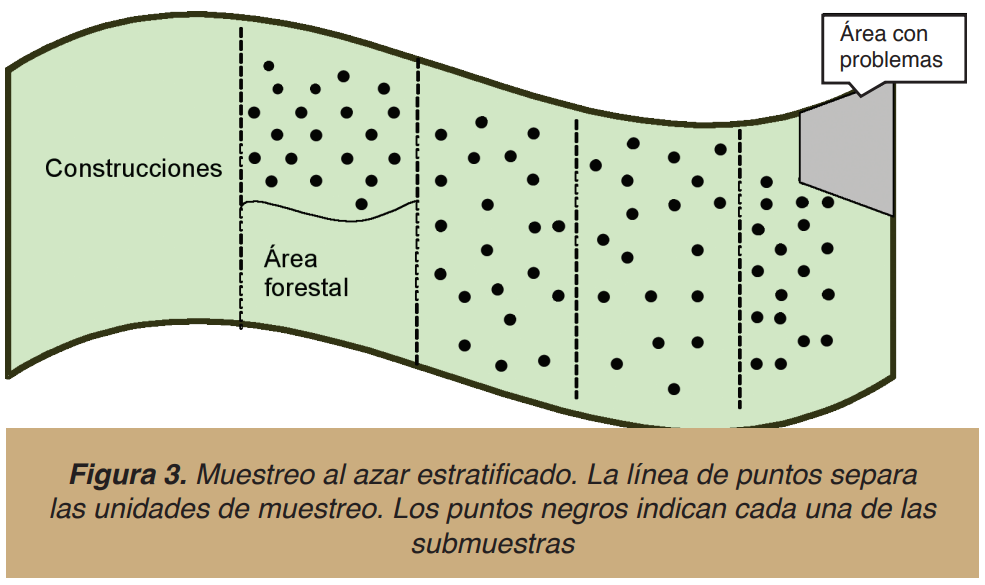
\includegraphics[width=0.3\paperwidth]{ref/stratified-sampling-examples.png}
    \caption{Ejemplo de estratos para diagnóstico de fertilidad}
    Fuente: Muestreo y Análisis de Suelos para Diagnóstico de Fertilidad \cite{lassaga-2011}
\end{figure}

Como resumen de los tipos de muestreos de utilidad se puede ilustrar el siguiente ejemplo:

\begin{figure}[H]
    \centering
    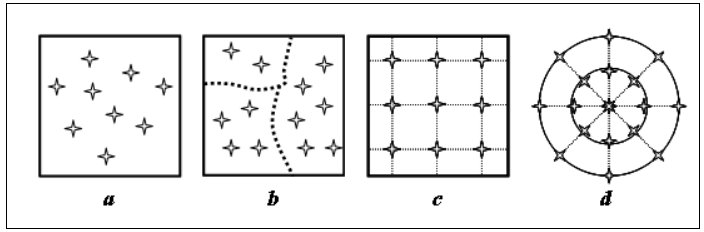
\includegraphics[width=0.3\paperwidth]{ref/kind-of-samplings-example.png}
    \caption{Ejemplo de tipos de muestreos. a) aleatorio simple, b) aleatorio estratificado, c) sistemático rejilla rectangular, d) sistemático rejilla polar}
    Fuente: Gobierno de México $\mid$ INNEC Instituto Nacional de Ecología y Cambio Climático \cite{innec-2007}
\end{figure}

Sea $S_h$ el conjunto de $n_h$ unidades para el estrato $H$. El valor de la unidad \textit{j}-ésima en el estrato $H$ se define como $x_{hj}$. Se siguen las siguientes valoraciones para el muestreo estratificado \cite{lohr-2009}:

\bigbreak

\textbf{Población total en el estrato H}
\bigbreak
$t_h = \sum \limits_{j=1}^{N_h} x_{hj}$


\bigbreak

\textbf{Total de la población}
\bigbreak
$t = \sum \limits_{h=1}^H t_h$


\bigbreak

\textbf{Media de la población para el estrato $H$}
\bigbreak
$\overline{x}_{hU} = \frac{\sum \limits_{j=1}^{N_h} x_{hj}}{N_h} = \frac{t_h}{N_h}$


\bigbreak

\textbf{Media de la población en general}
\bigbreak
$\overline{x}_U = \frac{\sum \limits_{h=1}^H \sum \limits_{j=1}^{N_h} x_{hj}}{N} = \frac{t}{N}$


\bigbreak

\textbf{Varianza de la población en el estrato $H$}
\bigbreak
$S_h^2 = \sum \limits_{j=1}^{N_h} \frac{(x_{hj} - \overline{x}_{hU})^2}{N_h - 1}$


\bigbreak

A partir de aquí, otros cálculos para los MAS se pueden aplicar para cada estrato. Se tiene que:

\bigbreak

$\overline{x}_h = \frac{1}{n_h} \sum \limits_{j \in S_h} x_{hj}$

\bigbreak

$s^2_h = \sum \limits_{j \in S_h} \frac{(x_{hj} - \overline{x}_h)^2}{n_h - 1}$

\bigbreak

El muestreo estratificado sin reemplazo basado en el MAS es el objetivo principal para obtener resultados bajo este marco teórico.

\subsubsection{Varianza}

Asumiendo que se tiene un muestreo estratificado donde cada estrato es relativamente homogéneo, la varianza de cada estrato es pequeña por lo que la varianza del estimado final también será pequeña, por consiguiente se sigue que \cite{gulland-1966}:

\bigbreak

Tenemos siempre que $N$ es el total de la población, $N_h$ es el $H$-ésimo estrato y $N=SN_h$. Una muestra de $n_h$ es tomada entonces del $H$-ésimo estrato, los valores que se desean estimar (longitud, peso, etc.) son dados por $x_{hj}$, $j=1,...,n_h$. De arriba, tenemos que la media estimada para el estrato $H$ es

$$
\overline{x}_h = \frac{1}{n_h} \sum \limits_{h=1}^{n_h} x_{hj}
$$

Un estimado sin sesgo de la media en toda la población es dado por esta media ponderada:

$$
\overline{x} = \frac{1}{N} \sum \limits_{h} N_h \overline{x}_h
$$

Si la varianza dentro del $H$-ésimo estrato es $S_h^2$

$$
var(\overline{x}_h) = \frac{1}{n_h} S_h^2
$$

y

$$
var(\overline{x}) = \frac{1}{N^2} \sum \frac{N_h^2}{n_h}S_h^2
$$

dado que $n_h$ sea pequeño comparado a $N_h$. Sino, las varianzas son dadas por

$$
var(\overline{x}_h) = \frac{1}{n_h}(1 - \frac{n_h}{N_h})S_h^2
$$


$$
var(\overline{x}) = \frac{1}{N^2} \sum \limits_h N_h^2 \frac{1}{n_h}(1 - \frac{n_h}{N_h})s_h^2 = \frac{1}{N^2} \sum \limits_h N_h (N_h - n_h) \frac{1}{n_h} S_h^2
$$

Esta varianza puede ser comparada con la varianza del estimado obtenido al hacer el muestreo aleatorio de la población total:

$$
var(\overline{x}') = \frac{1}{n}S^2
$$

o

$$
var(\overline{x}) = \frac{1}{n}(1 - \frac{n}{N})S^2
$$

si $n$ no es pequeño comparado con $N$ donde $S^2$ es la varianza de la población total.

\subsubsection{Ejemplo}

En esta subsección se presenta un ejemplo con datos reales obtenido del \textit{Manual of Sampling and Statistical Methods for Fisheries Biology} \cite{gulland-1966}:

\bigbreak

\subsubsection{Barco de pesca comercial}

La captura de un arrastrero comercial que desembarca eglefino \footnote{El eglefino es un miembro de la familia del bacalao con un sabor suave, carne firme y textura húmeda. Se usa indistintamente con el bacalao pero tiene un sabor ligeramente más dulce, lo que lo convierte en el mejor pescado blanco para ahumar. El eglefino se vende comúnmente fresco, congelado o ahumado \cite{sustainable-fishing-msc-marine-stewardship-council-2021}.} en Aberdeen \footnote{Aberdeen es una ciudad en Escocia \cite{wikipedia-aberdeen-2021}.} se clasificó en cuatro categorías de tamaño que forman los cuatro estratos. Se midieron muestras de eglefino de cada categoría y los datos resultantes se pueden resumir de la siguiente manera:

\bigbreak

% ----- TABLE

\begin{table}[H]
\centering
\begin{tabular}{|l|l|l|l|l|}
\hline
\rowcolor[HTML]{CBCEFB}
\multicolumn{1}{|c|}{\cellcolor[HTML]{CBCEFB}\textbf{Categoría}} & \multicolumn{1}{c|}{\cellcolor[HTML]{CBCEFB}\textbf{$N_h$}} & \multicolumn{1}{c|}{\cellcolor[HTML]{CBCEFB}\textbf{$n_h$}} & \multicolumn{1}{c|}{\cellcolor[HTML]{CBCEFB}\textbf{$Sx_{hj}$}} & \multicolumn{1}{c|}{\cellcolor[HTML]{CBCEFB}\textbf{$Sx_{hj}^2$}} \\ \hline
Pequeña                                                          & 2,432                                                        & 152                                                         & 5,284                                                            & 185,532                                                            \\ \hline
\rowcolor[HTML]{EFEFEF}
Pequeña-media                                                    & 1,656                                                        & 92                                                          & 3,817                                                            & 158,953                                                            \\ \hline
Media                                                            & 2,268                                                        & 63                                                          & 3,033                                                            & 146,357                                                            \\ \hline
\rowcolor[HTML]{EFEFEF}
Grande                                                           & 665                                                         & 35                                                          & 2,027                                                            & 118,169                                                            \\ \hline
\rowcolor[HTML]{FFCE93}
Total                                                            & 7,021                                                        & 342                                                         & 14,161                                                           & 609,011                                                            \\ \hline
\end{tabular}
\caption{Datos para cada estrato de la captura del barco de pesca}
\end{table}

% ----- END TABLE

donde $x$ es la longitud del pescado en $cm$.

Entonces usando como estimado de $S_h^2$ la ecuación:

$$
S_h^2 = \frac{1}{n_h - 1} \left[ \sum \limits_{h=1}^{N_h} x_{hj}^2 - \frac{1}{n_h} \left(\sum \limits_{h=1}^{N_h}x_{xj} \right)^2 \right]
$$

también tenemos que:

% ----- TABLE

\begin{table}[H]
\centering
\begin{tabular}{|l|l|l|l|l|l|}
\hline
\rowcolor[HTML]{CBCEFB}
\multicolumn{1}{|c|}{\cellcolor[HTML]{CBCEFB}\textbf{Categoría}} & \multicolumn{1}{c|}{\cellcolor[HTML]{CBCEFB}\textbf{$x_h$}} & \multicolumn{1}{c|}{\cellcolor[HTML]{CBCEFB}\textbf{$N_hx_h$}} & \multicolumn{1}{c|}{\cellcolor[HTML]{CBCEFB}\textbf{$S_{h}^2$}} & \multicolumn{1}{c|}{\cellcolor[HTML]{CBCEFB}\textbf{$\frac{S_{h}^2}{n_h}$}} & \textbf{$\frac{N_h^2S_h^2}{n_h}$} \\ \hline
Pequeña                                                          & 34.763                                                      & 84,544                                                         & 12.21                                                           & 0.0803                                                                      & 474,900                           \\ \hline
\rowcolor[HTML]{EFEFEF}
Pequeña-media                                                    & 41.489                                                      & 68,706                                                         & 6.47                                                            & 0.0703                                                                      & 192,800                           \\ \hline
Media                                                            & 48.143                                                      & 109,188                                                        & 5.48                                                            & 0.0870                                                                      & 447,500                           \\ \hline
\rowcolor[HTML]{EFEFEF}
Grande                                                           & 57.914                                                      & 38,513                                                         & 22.85                                                           & 0.6529                                                                      & 288,700                           \\ \hline
\rowcolor[HTML]{FFCE93}
Total                                                            &                                                             & 300,951                                                        &                                                                 &                                                                             & 1,403,900                         \\ \hline
\end{tabular}
\end{table}

% ----- END TABLE

Así:

\bigbreak

$\overline{x} = \frac{300,951}{7,021} = 42.9$

\bigbreak

$var(\overline{x}) = \frac{300,951}{(7,021)^2} = 0.0285$

\bigbreak

$s.d(\overline{x}) = 0.17$

\bigbreak

El $95\%$ de confianza para la longitud media real del pescado establece dicho intervalo en $42.9 \pm (2 \cdot 0.17)$ esto es, $42.6-43.2 \, cm$.
